\documentclass{homework}

\title{Final Problems}
\author{Kevin Evans}
\studentid{11571810}
\date{May 5, 2021}
\setclass{Physics}{461}
\usepackage{amssymb}
\usepackage{mathtools}

\usepackage{amsthm}
\usepackage{amsmath}
\usepackage{slashed}
\usepackage{relsize}
\usepackage{threeparttable}
\usepackage{float}
\usepackage{booktabs}
\usepackage{boldline}
\usepackage{changepage}
\usepackage{physics}
\usepackage[inter-unit-product =\cdot]{siunitx}
\usepackage{setspace}

\usepackage[makeroom]{cancel}
%\usepackage{pgfplots}

\usepackage{enumitem}
\usepackage{times}
\usepackage{mhchem}

\usepackage{calligra}
\DeclareMathAlphabet{\mathcalligra}{T1}{calligra}{m}{n}
\DeclareFontShape{T1}{calligra}{m}{n}{<->s*[2.2]callig15}{}
\newcommand{\scriptr}{\mathcalligra{r}\,}
\newcommand{\boldscriptr}{\pmb{\mathcalligra{r}}\,}
\newcommand{\emf}{\mathcal{E}}

\begin{document}
	\maketitle
	\section{Laser cooling, Sisyphus effect, and the magneto-optical trap}
	\subsubsection*{Laser cooling}
	Optical cooling is a method of cooling an atomic beam using a laser beam. If we have an atomic beam propagating in $z$, consisting of atoms of mass $m$ and velocity $v$, we can point a laser against the direction of the atomic beam. This laser would contain photons carrying momentum $\hbar k$. As the atoms and photons ``collide,'' the conserved total momentum is given by $$\bvec{p} = m \bvec{v} + \hbar \bvec{k}.$$
	Since the atom and photons were traveling in opposite directions, the atom now has decreased slightly in velocity with
	$$\Delta v = \hbar k / m = h \nu / m c.$$
	This mechanism requires light of an exact resonance frequency, where the atom absorbs photons that match this condition. As the atom absorbs the photon, the atom increases in energy from $\ket{1} \to \ket{2}$. As the state decays back to the lower state $\ket{1}$, the atom emits a photon in a random direction. Over several iterations of this absorption-emission process, the time average change in momentum due to emission is zero.
	
	For an atomic gas, the atoms are moving in random directions with various velocities, but the average velocity over an ensemble of atoms is zero. If we use a red-detuned laser---where the laser's energy is lower than the transition energy---and point it toward this atomic gas, this will excite the atoms that are moving toward the direction of the laser (against the laser's propagation). This is the basis for Doppler shifting. In practice, diode lasers can be shifted by adjusting the diode current to shift the laser frequency, following the condition
	$$\omega = \omega_0 - k v,$$
	where $\omega_0$ is the optical transition frequency. As the atoms slow to lower temperatures, the transition frequency changes and the laser frequency will need to be adjusted continually---a method known as \textit{chirp cooling}. 
	
	Alternatively, instead of employing chirp cooling, the energy levels of the atoms can be changed using the Zeeman effect with a magnetic field gradient. By applying a gradient, this will ensure the laser stays resonant.
	
%	This method of \textit{Doppler cooling} is capable of reaching limits of \SI{10}{\micro\K}.
%	TODO
	
	The method described above will cool atoms moving in a single direction. To slow the atoms from all directions, the solution is clear: add more lasers! In practice, laser cooling consists of three counter-propagating pairs of perpendicular lasers with the cooled atoms placed where the beams intersect, creating an \textit{optical molasses}. This is shown in Figure \ref{fig:finaloptmol} below.
	% TODO: \usepackage{graphicx} required
	\begin{figure}[H]
		\centering
		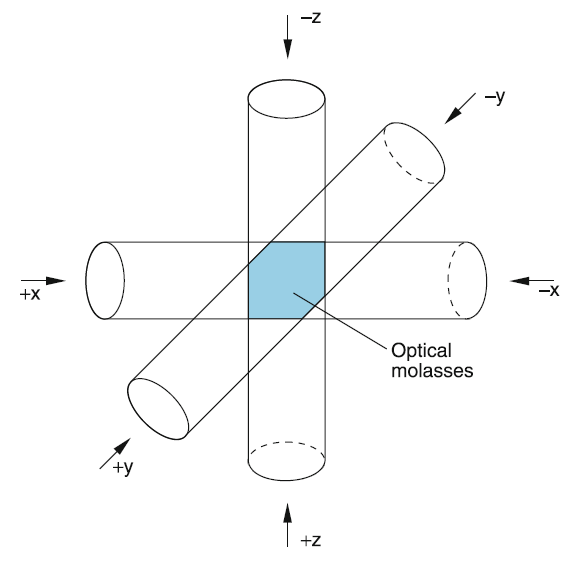
\includegraphics[width=0.5\linewidth]{final_optmol}
		\caption{Three pairs of counterpropagating beams, intersecting at the center of the trap. (Source: Demtr\"oder, p. 455.)}
		\label{fig:finaloptmol}
	\end{figure}
	
	The broadened absorption probability can be described as a Lorentzian,
	$$P(\omega) = \frac{P_0(\gamma / 2)^2}{(\omega_L - \omega_0 - \bvec{k} \cdot \bvec{v})^2 + (\gamma / 2)^2}.$$
	Here, the probability is a function of the light's propagation $\bvec{k}$ and $\omega$, the natural linewidth $\omega_L$, atomic resonance frequency $\omega_0$, and particle velocity $\bvec{v}$. For a pair of counter-propagating lasers, the absorption rates is 
	$$R^\pm(v) = \frac{R_0}{1 + \left[\omega_L - \omega_0 \pm \bvec{k} \cdot \bvec{v} / (\gamma / 2)\right]^2}.$$ For each axis $i$, the total recoil force can be shown to equal \begin{align*}
		\bvec{F}_i & = -\left[R^+(v_i) - R^-(v_i)\right] \hbar \bvec{k} \\
			& = \frac{16R_0 \delta k v \hbar k}{\gamma^2 \left[
					1 + \frac{8}{\gamma^2} \left( \delta^2 + (kv)^2\right)
					+ \left(\frac{\delta^2 - (kv)^2}{\gamma^2 / 4} \right)^2
				\right]}.
	\end{align*}
	In the approximation $kv \ll \omega_L - \omega_0 = \delta$, this reduces to
	$$\bvec{F}_i = a \bvec{v}_i,$$
	where
	$$a \approx \frac{16 \delta \hbar k^2 R_0}{\gamma^2 \left[1 + (2 \delta / \gamma)^2\right]^2}.$$
	% Doppler shift pp 8 https://web.stanford.edu/~rpam/dropoff/Phys041N/lecture6-lasercooling.pdf
	
	\subsubsection*{Sisyphus cooling}
	In Sisyphus cooling, an optical lattice is constructed with an array of $\sigma^+$ and $\sigma^-$ polarized light. In this optical lattice, the regions alternate between $\sigma^+$, $\sigma^-$, and linearly-polarized light (where there is no phase difference). If we consider an alkali atom with ground state $J=1/2$ and excited state $J'=3/2$, each will have degenerate energy levels. In the presence of a light wave, the degeneracy is lifted by the AC Stark Effect and the energy levels now become a function of the light polarization. Combined with the selection rules that govern atomic transitions, atoms can be optically pumped to higher states then will fall down to a ground state with lower energy.
	
	In this alkali atom scenario, initially at $M_J=-1/2$, it $\sigma^+$ (right-hand) polarized light is incident on it, the atom can absorb the photon and be excited to the $M_{J'}=1/2$ state\footnote{Is this action equivalent to the raising and lowering operators?}. From here, it can either fall back down to the original $M_J=-1/2$ state or it can fall to the $M_J=1/2$ state. The difference between these two transitions is: if it falls to the original $M_J=-1/2$ state, the cycle can repeat again. If it falls to $M_J=1/2$, the atom is stuck in this state unless $\sigma^-$ light is applied, as $\sigma^+$ absorption would require a higher angular momentum state\footnote{This was described in-class as being ``pumped to extreme levels.''}.
	
	Due to the AC Stark effect, these two states have different energy levels depending on the $M_J$ value. This is the \textit{light shift} and is shown graphically in Figure \ref{fig:finalsisy}.

	\begin{figure}[h]
		\centering
		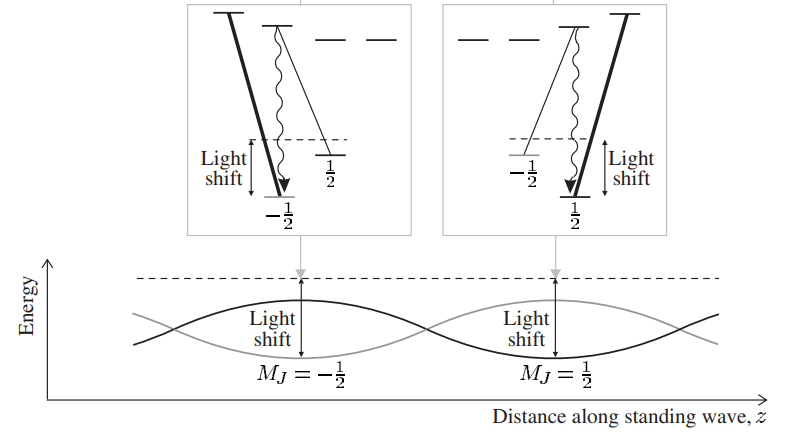
\includegraphics[width=0.7\linewidth]{final_sisy}
		\caption{The light shift created by the AC Stark effect. (Source: the class website)}
		\label{fig:finalsisy}
	\end{figure}
	
	\subsubsection*{Magneto-optical trapping}
	In a magneto-optical traps (MOT), optical cooling is combined with a magnetic trap, allowing neutral atoms to be cooled to limits of several microkelvin. A pair of anti-Helmholtz coils creates a magnetic field that is zero at the center of the trap, and increases linearly as the distance, $$B(z) = B_0 z.$$
	From the Zeeman effect, the energies of trapped atoms now split as $$E_i = - \bvec{p}_m \cdot \bvec{B} = g_F \mu_B m_F \abs{B_0 z},$$
	where $F$ is the total angular momentum quantum number. As the magnetic field is proportional to $z$, the energy will have the same proportionality.
	
	Additionally, the MOT has three sets of counter-propagating perpendicular laser beams with circular polarization. These beams are red-detuned, following 
		$$\delta \equiv \omega_0 - \omega > 0.$$
	By red-tuning the laser, atoms at the center of the trap are dark to the laser and the optical transitions are not induced. If the atoms move outward toward $\pm z$ away from the origin, they will encounter $\sigma^\pm$ light and will be recoiled back toward the center. This action confines atoms to the center of the MOT.  Additionally, this causes Doppler cooling, as discussed earlier in this problem. The force acting on the atoms is $$\bvec{F} = R_{\sigma^+}(z) \hbar \bvec{k}_{\sigma^+} + R_{\sigma^-}(z)z \hbar \bvec{k}_{\sigma^-}$$
	where for a Lorenzian absorption profile, the absorption rates are given as
	$$R_{\sigma^\pm} = \frac{R_0}{1 + \left[\frac{\omega_L - \omega_0 \pm p_m B_0 z / \hbar}{\gamma / 2}\right]^2}.$$
	The restoring force can be approximated for $z \to 0$ as 
	$$
		F_z = - D z \quad \text{where} \quad D = R_0 p_m B_0 \frac{16 k \delta}{\gamma^2(1 + 4 \delta^2 / \gamma^2)^2}.
	$$
	The net force on the atom then consists of a spatially-dependent term and a term which depends on the velocity,
	$$F_z = - D z - a v_z.$$
	\pagebreak
	
	\section{Einstein A and B coefficients}
	Consider an atom with two states, a lower state $\ket{1}$ and excited state $\ket{2}$. The lower and excited states have population $N_1$ and $N_2$ respectively. These states are separated by an optical transition with energy
	$$\Delta E = E_2 - E_1 = h \nu.$$
	We can take three mechanisms for transitions: absorption of a photon, induced emission, and spontaneous emission. Both the absorption and induced emission require an energy source to trigger the mechanism, which will be an electromagnetic radiation field with spectral energy density $w(\nu)$.
	
	The absorption rate and induced emission rate can be expressed as a function of an Einstein coefficient, state population, and the spectral energy density \begin{align*}
		\mathrm{Rate}_{1 \to 2}^\mathrm{abs} & = B_{12} N_1 w(\nu) \\
		\mathrm{Rate}_{2 \to 1}^\mathrm{ind} & = B_{21} N_2 w(\nu).
	\end{align*}
	The spontaneous emission happens spontaneously and does not depend on the incident light, 
	$$\mathrm{Rate}_{2 \to 1}^\mathrm{spont} = A_{21} N_2.$$
	Balancing these rates, we can find the relationship between the Einstein coefficients \begin{align*}
		B_{12} N_1 w(\nu) & = A_{21} N_2 + B_{21} N_2 w(\nu)  \\
			& = N_2 \left[ A_{21} + B_{21} w(\nu) \right]
	\end{align*}
	The relationship between the populations follows the Boltzmann distribution \begin{align*}
		\frac{N_2}{N_1} & = \frac{g_2}{g_1} e^{-h \nu / k_B T},
	\end{align*}
	where $g_1$ and $g_2$ are the statistical weights (degeneracy) of each state. From these two relationships, 
	\begin{align*}
		\frac{N_2}{N_1} & = \frac{B_{12} w(\nu)}{A_{21} + B_{21} w(\nu)} = \frac{g_2}{g_1} e^{-h \nu / k_B T} \\
			& = \frac{B_{12} / B_{21}}{1 + A_{21} / B_{21} w(\nu)} \\
		\Rightarrow w(\nu) & = \frac{A_{21} / B_{21}}{(g_1 / g_2) (B_{12} / B_{21}) e^{h \nu / k_B T} - 1}.
	\end{align*}
	The spectral energy density can be equated to Planck's blackbody law, where 
		$$w(\nu) = \frac{8 \pi h \nu^3}{c^3} \frac{1}{e^{h \nu / k_B T} - 1}.$$
	This presents the relationship between the Einstein coefficients, \begin{align*}
		B_{21} & = \frac{g_1}{g_2} B_{12} \\
		A_{21} & = \frac{8 \pi h \nu^3}{c^3} B_{21}.
	\end{align*}
	For systems with equal statistical weights, $g_1 = g_2$ and $$B_{12} = B_{21}.$$
	
	\pagebreak
	
	\section{Solid-state lasers}
	To begin this problem, I'll be first introducing lasers and providing a little handwavy background. I'm hoping to explain the background once, so I won't need to explain terms again when discussing gas lasers in Problem 4.
	
	\subsubsection*{Background on lasers}
	Lasers are a method of leveraging stimulated emission to produce high intensity, coherent light. Lasers consist of three main components: the active medium where stimulated emission occurs, an energy pump that generates population inversion in the active medium, and a optical resonator cavity. Population inversion occurs when atoms of the active medium in the excited state $\ket{i}$ exceeds the atoms in the ground state $\ket{k}$, contrary to thermal equilibrium, i.e. $$N_i > \frac{g_i}{g_k} N_k.$$
	Under this condition, the Beer's absorption law coefficient $\alpha$ becomes negative, as
	\begin{align*}
		\alpha(\nu) & = \left[ N_k - (g_k / g_i) N_i\right] \sigma(\nu).
	\end{align*}
	Applying this to Beer's absorption law $$I(\nu, z)  = I_0 e^{-\alpha(\nu) z},$$
	a negative coefficient $\alpha$ implies the intensity increases under population inversion. Taking into account all losses internal to the laser of length $L$ as a frequency-dependent factor $\gamma(\nu)$, the gain of the laser is $$G(\nu) = \frac{I(\nu, 2L)}{I(\nu, 0)} = e^{-(2 \alpha(nu) L + \gamma(\nu))}.$$
	For lasing to occur, $G(\nu)>1$ where the gain exceeds any internal losses and light can oscillate across the laser cavity. From these two conditions, lasing occurs when the population is inverted such that $$\boxed{N_i(g_k / g_i) - N_k \ge \frac{\gamma(\nu)}{2 \sigma(\nu) L}.}$$
	\textit{Photon avalanche} occurs where a photon (either by another stimulated photon or by the energy pump) induces another atom to undergo stimulated emission as it travels across the active medium. This creates a cycle where the stimulated photons exponentially induce emission as they travel across the medium.
	$$\cdots$$
	
	Previously, the threshold condition for achieving lasing was discussed. Now we'll describe how population inversion is achieved. Earlier, a two-level system was used to give background on lasing. However, two-level lasing is not feasible since when we excite the system, both levels will be at most equally populated and population inversion is not possible\footnote{I'm pretty sure this is because the Einstein $B$ coefficients are equal, as in the induced coefficient $B_{21}$ equals the absorption coefficient $B_{12}$ (given equal statistical weights). But this might be wrong and I'm misunderstanding it.}. Therefore, a third intermediate metastable step is required.

	
	\subsubsection*{Solid-state active media}
	Solid-state lasers are one of the earliest methods of producing laser, with Maiman demonstrating a ruby laser in 1960.  Solid-state lasers rely on a glass or single crystal, typically doped with atoms that can be optically pumped to excited states. 
	
	In a ruby laser, an aluminum oxide (\ce{Al2O3}) crystal is doped with $\approx 1\%$ Chromium (\ce{Cr+++}) ions. In early ruby lasers, the ions are pumped to the higher energy state using a helical flash lamp that surrounds the crystal rod. Ruby lasers can be treated as a three-level laser, where a flashlamp pumps ions to a broadened excited state $E_1$. These ions can emit phonons to the crystal lattice, resulting in a fast radiationless decay to an intermediate energy $E_i$. From the intermediate energy $E_i$, the system can fall back to the ground state $E_0$, emitting a photon across the crystal. This process is shown in Figure \ref{}.
	
	\section{Gas lasers}
	Gas lasers operate with a gas as the active media. Typically, an electric discharge is used as the pumping mechanism where electrons collide with the gas atoms. As an example, we will discuss the helium-neon (He-Ne) laser, a common gas laser. 
	
	Population inversion is accomplished by a small current discharging across the low-pressure gas mixture. In this process, electrons inelastically collide with the helium raising from the ground $n=1$ state to one of two metastable $n=2$ states: \ce{2^3 S_1} and \ce{2^1 S_0}. These two states of helium have similar resonances to two levels in neon: \ce{5 S_2} and \ce{4 S_2}, and the helium atoms transfer collisional energy to these two states. This can be described as
	\begin{align*}
		\ce{He^* (2^1 S_0)} + \ce{Ne (2^1 S_0)} & \quad \to \quad \ce{He(1^1 S_0)} +  \ce{Ne^* (5s)} + \Delta E \\
		\ce{He^* (2^3 S_0)} + \ce{Ne (2^1 S_0)} + \Delta E & \quad \to \quad  \ce{He(1^1 S_0)} +  \ce{Ne^* (4s)} 
	\end{align*}
	where $^*$ represents an excited state, and $\Delta E$ is a small ($<\SI{0.1}{\eV}$) difference between the two states and is supplied by the kinetic energy of the atoms. This process creates a population inversion on the $4s$ and $5s$ energies, as the $3s$ level is vacant. As energies fall to the $3s$ state by photon emission, three wavelengths are possible: \begin{align*}
		5s \to 4s & \qquad \SI{3.39}{\um} \\
		4p \to 3p & \qquad \SI{1.15}{\um} \\
		5s \to 3p & \qquad \SI{663}{\nm}.
	\end{align*}
	Once in the $n=3$ state, the gas collides with the walls of the resonator cavity and energy is lost through radiationless processes. As there are now two excited states, this is a \textit{four-level system}.
	
	
	\pagebreak
	
	\section{A brief introduction to the Gross-Pitaevskii equation}
	The Gross-Pitaevskii equation (GPE) is a non-linear Schr\"odinger equation that models a density of Bose-Einstein condensates (BECs). The GPE includes a non-linear term that addresses particle interaction through a mean-field approximation. 
	The GPE makes several assumptions: (1) temperatures are driven lower than the critical temperature $T_c$, i.e. it is a BEC, (2) interactions are weak and it [TODO], (3) the many-body wavefunction can be approximated by a single-particle wavefunction. Without these assumptions, an exact parameterized wavefunction of many particles would not be feasible to work with due to its complexity. We can assume a macroscopic wavefunction of the form
	$$\Psi(\bvec{r}, t) = \sqrt{n(\bvec{r}, t)} e^{iS(\bvec{r}, t)},$$
	where $n(\bvec{r}, t)$ is the density and $S(\bvec{r}, t)$ is the phase distribution of the BEC.
	The time-dependent GPE is
	$$i \hbar \pdv{\Psi}{t} = - \frac{\hbar^2}{2m} \laplacian{\Psi} + V(\bvec{r}, t) \Psi + g \abs{\Psi}^2 \Psi,$$
	where the coefficient $g$ is
	$$g = \frac{4 \pi \hbar^2 a_s}{m}.$$
	In this constant, $a_s$ is the s-wave scattering length\footnote{I don't fully understand \textit{what} $a_s$ is, aside from a value that's assigned given potentials in an atom.}, which depends on the atomic species and can be positive or negative, depending if the interaction is attractive ($g<0$) or repulsive ($g>0$, the typical sign). This cubic term gives an energy contribution due to the mean-field interactions of all other atoms in space and can be controlled in experiments with Feshbach resonances. With $g=0$, we have the regular ol' single-particle Schr\"odinger equation. 
	
	As this is a many-body system of $N$ atoms, we have a normalization condition where 
	$$\int \abs{\Psi}^2 \dd[3]{\bvec{r}} = N.$$
	The total mass of the condensate is then $M=mN$. The energy is given by the expression
	$$E = \int \left[ \frac{\hbar^2}{2m} \abs{\grad{\Psi}}^2 + V\abs{\Psi}^2 + \frac{g}{2} \abs{\Psi}^4\right] \dd[3]{\bvec{r}} = E_\mathrm{kin} + E_\mathrm{pot} + E_\mathrm{int}.$$ Here, $E_\mathrm{int}$ is the interaction energy. Time-independent solutions of the GPE should satisfy
		$$\Psi(\bvec{r}, t) = \psi(\bvec{r}) e^{-i \mu t / \hbar},$$
	where $\mu$ is a constant chemical potential, $\pdv*{E}{N}$.
	This is analogous to the energy in the time-independent Schr\"odinger equation. Inserting this solution into the GPE results in the \textit{time-independent GPE}, 
	$$\mu \psi = -\frac{\hbar^2}{2 m} \laplacian{\psi} + V(\bvec{r}) + g \abs{\psi}^2 \psi.$$
	This implies that $$\mu = \frac{1}{N} \left( E_\mathrm{kin} + E_\mathrm{pot} + E_\mathrm{int}\right).$$
	
	There are several exact solutions to the GPE but each have limitations. Typically, numeric methods are employed to find solutions to the GPE. A simple solution\footnote{This solution does not actually describe a BEC due to an energy gap, although it is a valid solution to the GPE.} to the GPE is a plane wave $$\Psi(\bvec{r}) = \sqrt{\frac{N}{V}}e^{i\bvec{k} \cdot \bvec{r}}.$$
	For a one-dimensional condensate near a hard wall (i.e. a one-sided well), we can define a potential $$V(x) = \begin{cases}
		\infty & x < 0 \\
		0 & x \ge 0,
	\end{cases}$$
	and an initial condition $\psi_0 = \psi(0) = 0$. Another condition can be
	
	$$\lim_{x \to \infty} \psi(x) = \sqrt{\mu / g},$$
	implying the condensate ``recovers'' as it moves away from the wall. Within the well, the one-dimensional GPE is
	$$\mu \psi = -\frac{\hbar^2}{2m} \pdv[2]{\psi}{x} + g\abs{\psi}^2 \psi.$$ The solution to this equation with these boundary conditions is
	$$\psi(x) = \psi_0 \tanh(\frac{x}{\xi}).$$
	In the context of GPEs, $\xi$ is the \textit{healing length}, $$\xi = \frac{\hbar}{\sqrt{mn_0 g}}.$$ This length gives $x$ a characteristic distance which it changes spatially, i.e. giving the order of magnitude of the wavefunction. 
%	\nocite{*}
%	\bibliographystyle{unsrt}
%	\bibliography{mybib}
%	
\end{document}